\chapter{Vorwissen}\label{ch:Kapitel00}
Diese Unterlagen behandeln anspruchsvolle Inhalte der Informatik und Mathematik. Um ihnen gerecht zu werden, bedarf es einer mathematisch präzisen Ausdrucksweise. Den überwiegenden Teil der benötigten mathematischen Werkzeuge werden die Lesenden typischerweise in den ersten Jahren des Gymnasiums kennengelernt haben. Einige der von uns benötigten Konzepte werden den meisten Lesenden jedoch vermutlich noch nicht bekannt sein. Diese Konzepte wollen wir in diesem Kapitel einführen. Wir werden dies in kompakter Form tun und an verschiedenen Stellen auf artifiziell wirkende (forcierte) Beispiele bewusst verzichten.

\section{Mathematik}
\subsection{Direkter und indirekter Beweis}
Seien $A$ und $C$ mathematische Aussagen. Wir möchten beweisen, dass die Aussage
\begin{align*}
    A\Rightarrow C
\end{align*}
($A$ impliziert $C$) gilt. Solch ein Beweis kann im Wesentlichen auf zwei Arten erbracht werden: entweder durch einen \tib{direkten Beweis}\index{Beweis!direkter} oder einen \tib{indirekten Beweis}\index{Beweis!indirekter}.

\subsubsection{Direkter Beweis}
Der direkte Beweis macht von folgender logischen Tatsache Gebrauch: Impliziert $A$ eine weitere Aussage $B$
\begin{align*}
    A \Rightarrow B
\end{align*}
und $B$ impliziert wiederum $C$:
\begin{align*}
    B \Rightarrow C,
\end{align*}
dann impliziert $A$ auch $C$. Zusammengefasst gilt also:
\begin{align}\label{eq:direkterBeweis}
     \lr{\textcolor{Blue}{(A\Rightarrow B) \text{ und } (B\Rightarrow C)}} \Rightarrow \lr{\textcolor{Green}{A\Rightarrow C}}.
\end{align}
Um die Richtigkeit der Implikation $A\Rightarrow C$ zu beweisen, zerlegt man die Implikation in bereits als für richtig befundene \enquote{Teilaussagen} $A\Rightarrow B$ und $B\Rightarrow C$, also
\begin{align*}
    \textcolor{Blue}{(A\Rightarrow B) \text{ und } (B\Rightarrow C)}.
\end{align*}
Danach folgt die Implikation $\textcolor{Green}{A\Rightarrow C}$ aus Ausdruck \ref{eq:direkterBeweis}. Diese Strategie kann wiederholt angewendet werden und man erhält eine \enquote{Kette} logischer Implikationen (Schlüsse):
\begin{align*}
    \lr{ \textcolor{Blue}{(A\Rightarrow B_1) \text{ und } (B_1\Rightarrow B_2) \text{ und } (B_2\Rightarrow B_3) \text{ und } \ldots \text{ und } (B_n\Rightarrow C)} } \Rightarrow (\textcolor{Green}{A\Rightarrow C}).
\end{align*}
Dabei können die Begründungen der Implikationen $A\Rightarrow B_1$, $B_n\Rightarrow C$ sowie $B_k\Rightarrow B_{k+1}$ für jedes $k\in\lrc{1,2,\ldots, n-1}$ als logische \enquote{Zwischenschritte} verstanden werden.

\subsubsection{Indirekter Beweis}
Ein indirekter Beweis (Beweis durch Widerspruch) beginnt mit der Annahme, dass die Aussage $C$ falsch sei, dass also $\neg{C}$ (nicht $C$) richtig ist. Nun wird einzig, unter Verwendung der Richtigkeit von $A$ und $\neg{C}$ sowie bereits als wahr erkannter mathematischer Aussagen, die Richtigkeit einer Aussage $B$ abgeleitet, von der bereits bekannt ist, dass sie falsch ist. Dadurch haben wir einen \enquote{Widerspruch} erhalten und können folgern, dass $\neg{C}$ nicht richtig sein kann und somit $C$ wahr sein muss. Damit ist, wie gewünscht, die Implikation $A\Rightarrow C$ nachgewiesen.

\subsection{Kontraposition}
Seien $A$ und $B$ mathematische Aussagen. Logisch äquivalent zur Behauptung $A\Rightarrow B$ ist die Aussage $\neg{B}\Rightarrow \neg{A}$, welche \tib{Kontraposition}\index{Kontraposition} der Implikation $A\Rightarrow B$ genannt wird. Der Beweis für $A\Rightarrow B$ ist demnach auch erbracht, falls man zeigen kann, dass aus der Annahme, die Folgerungen seien nicht erfüllt, folgt, dass auch die Voraussetzungen nicht erfüllt sein können. Gelegentlich fällt es einem leichter, die Kontraposition $\neg{B}\Rightarrow \neg{A}$ einer Implikation $A\Rightarrow B$ zu zeigen.

\beispiel{-}
{Sei $A$ die Aussage \enquote{Es hat geregnet.} und $B$ die Aussage \enquote{Die Strasse ist nass.}. Die Implikation $A\Rightarrow B$ bedeutet: \enquote{Falls es geregnet hat, ist die Strasse nass.}

\noindent
Falls die Strasse nass ist, muss das umgekehrt nicht bedeuten, dass es geregnet hat. Beispielsweise könnte die Strasse auch von der Strassenreinigung nass gemacht worden sein. Was wir aber sicherlich sagen können, ist, dass falls die Strasse \textit{nicht} nass ist, es auch \textit{nicht} geregnet haben kann, was genau 
$\neg{B}\Rightarrow \neg{A}$ bedeutet.
}

\subsection{Funktionen}
\subsubsection{Definition einer Funktion (*)}
\begin{definition}[Funktion als Vorschrift]{definition:funktion}
Seien $X$ und $Y$ Mengen. Wir sagen, dass eine \tib{Funktion}\index{Funktion} auf $X$ mit Werten in $Y$ definiert ist, wenn aufgrund einer \textit{Vorschrift} (\textit{Regel}) $f$ jedem Element $x\in X$ genau ein Element $y\in Y$ zugehörig ist.
\end{definition}
Wir sagen dann, dass die Menge $X$ die \tib{Definitionsmenge}\index{Funktion!Defintionsmenge einer} der Funktion ist.

Das Symbol $x$, das benutzt wird, um ein allgemeines Element dieser Menge zu beschreiben, wird \tib{Argument}\index{Funktion!Argument einer} oder \textit{unabhängige Variable} der Funktion genannt.

Das Element $y_0\in Y$, das einem Argument $x_0\in X$ zugeordnet wird, wird \tib{Wert}\index{Funktion!Wert einer} der Funktion in $x_0$ genannt oder auch Wert der Funktion an der Stelle $x = x_0$ und $f(x_0)$ geschrieben. Die Menge $Y$ wird \tib{Zielmenge}\index{Funktion!Zielmenge einer} der Funktion genannt.

Bei Änderung der Argumente $x\in X$ verändern sich im Allgemeinen die Resultate $y = f(x)\in Y$ in Abhängigkeit von den Werten $x$. Aus diesem Grund wird die Grösse $y=f(x)$ oft auch \textit{abhängige Variable} genannt.
\begin{definition}[Bild einer Funktion]{definition:bild}
Die Menge
\begin{align*}
    \text{im}\lr{f} := \setct{y\in Y}{es existiert ein $x\in X$ mit $y=f(x)$}
\end{align*}
von Werten, die von einer Funktion $f$ für alle Elemente in der Menge $X$ angenommen werden, wird \tib{Bild} (englisch: \textit{image}) oder \textit{Wertemenge} der Funktion $f:X\to Y$ genannt. Häufig wird $\text{im}\lr{f}$ alternativ als $f(X)$ geschrieben, wobei $X$ die Definitionsmenge von $f$ ist.
\end{definition}

\subsubsection{Surjektion, Injektion, Bijektion}
In diesen Unterlagen werden wir häufig über Funktionen sprechen. Insbesondere werden wir die folgenden drei Eigenschaften von Funktionen mehrmals verwenden.
\begin{definition}[surjektiv, injektiv, bijektiv]{definition:eigenschaftenFunktionen}
Seien $X$ und $Y$ Mengen und $f: X\to Y$ eine Funktion.
\begin{itemize}
    \item $f$ heisst \tib{surjektiv}\index{Funktion!surjektive} (eine \textit{Surjektion}), falls $\text{im}\lr{f} = Y$.
    
    \textcolor{Gray}{Intuitiv gesprochen, nimmt eine surjektive Funktion jeden Wert in der Zielmenge an. Zu beliebigem $y\in Y$ existiert (mindestens) ein $x\in X$, sodass $y=f(x)$.}
    \item $f$ heisst \tib{injektiv}\index{Funktion!injektive} (eine \textit{Injektion}), falls für $x_1,x_2\in X$ aus $x_1\neq x_2$ stets $f(x_1)\neq f(x_2)$ folgt.
    
    \textcolor{Gray}{Zwei verschiedene Eingaben erzeugen stets verschiedene Ausgaben.}
    \item $f$ heisst \tib{bijektiv}\index{Funktion!bijektive} (eine \textit{Bijektion}), falls $f$ sowohl surjektiv als auch injektiv ist.
    
    \textcolor{Gray}{Da $f$ surjektiv ist, existiert zu jedem $y\in Y$ ein $x\in X$ mit $f(x)=y$. Da $f$ injektiv ist, kann es kein anderes $\tilde{x}\in X$ mit $\tilde{x}\neq x$ geben, sodass $f(\tilde{x})=y$. Dadurch stellt eine Bijektion eine \enquote{Eins-zu-eins-Zuweisung} zwischen den Elementen aus $X$ und $Y$ dar.}
\end{itemize}
\end{definition}

\begin{figure}[H]
    \centering
    \begin{subfigure}[b]{0.30\textwidth}
        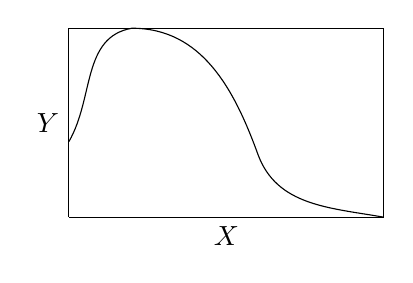
\begin{tikzpicture}[scale=0.8]
            \draw (0,0) -- node[below] {$X$} (5,0) -- (5,3) -- (0,3) -- node[left] {$Y$} (0,0);
            \draw (0,1.2) to [out=60,in=190] (1,3) to [out=360,in=110] (3,1) to [out=290,in=170] (5,0);
        \end{tikzpicture}
        \caption{surjektiv, nicht injektiv}
        \label{subfig:surjektiv}
    \end{subfigure}
    \begin{subfigure}[b]{0.30\textwidth}
        \begin{tikzpicture}[scale=0.8]
            \draw (0,0) -- node[below] {$X$} (5,0) -- (5,3) -- (0,3) -- node[left] {$Y$} (0,0);
            \draw (0,0.2) to [out=40,in=190] (5,2.5);
        \end{tikzpicture}
        \caption{injektiv, nicht surjektiv}
        \label{subfig:injektiv}
    \end{subfigure}
    \begin{subfigure}[b]{0.30\textwidth}
        \begin{tikzpicture}[scale=0.8]
            \draw (0,0) -- node[below] {$X$} (5,0) -- (5,3) -- (0,3) -- node[left] {$Y$} (0,0);
            \draw (0,0) to [out=15,in=250] (5,3);
        \end{tikzpicture}
        \caption{bijektiv}
        \label{subfig:bijektiv}
    \end{subfigure}%
    \caption{schematische Darstellung der Eigenschaften in \cref{definition:eigenschaftenFunktionen}}
    \label{fig:surinjbi}
\end{figure} 

\begin{figure}[H]
    \centering
    \begin{subfigure}[b]{0.30\textwidth}
        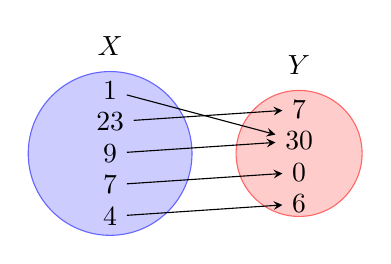
\begin{tikzpicture}[scale=0.8]
            % draw the sets
            \filldraw[fill=blue!20, draw=blue!60] (-1.5,0) circle (1.3cm);
            \filldraw[fill=red!20, draw=red!60] (1.5,0) circle (1cm);
            % the texts
            \node at (-1.5,1.7) {$X$};
            \node at (1.5,1.4) {$Y$};
            % the points in the sets (here I just create nodes to use them later on to position
            % the circles and the arrows
            \node (x1) at (-1.5,1.0) {$1$};
            \node (x2) at (-1.5,0.5) {$23$};
            \node (x3) at (-1.5,0.0) {$9$};
            \node (x4) at (-1.5,-0.5) {$7$};
            \node (x5) at (-1.5,-1.0) {$4$};
            
            \node (y1) at (1.5,0.7) {$7$};
            \node (y2) at (1.5,0.2) {$30$};
            \node (y3) at (1.5,-0.3) {$0$};
            \node (y4) at (1.5,-0.8) {$6$};
        
            % draw the arrows
            \draw[-stealth] (x1) -- (y2);
            \draw[-stealth] (x2) -- (y1);
            \draw[-stealth] (x3) -- (y2);
            \draw[-stealth] (x4) -- (y3);
            \draw[-stealth] (x5) -- (y4);
        \end{tikzpicture}
        \caption{surjektiv, nicht injektiv}
        \label{subfig:surjektivDiagramm}
    \end{subfigure}
    \begin{subfigure}[b]{0.30\textwidth}
        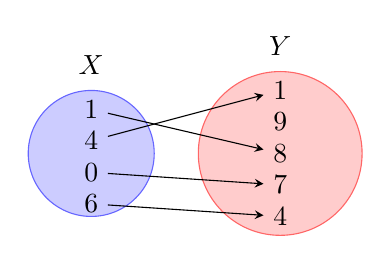
\begin{tikzpicture}[scale=0.8]
            \filldraw[fill=blue!20, draw=blue!60] (-1.5,0) circle (1cm);
            \filldraw[fill=red!20, draw=red!60] (1.5,0) circle (1.3cm);
        
            \node at (-1.5,1.4) {$X$};
            \node at (1.5,1.7) {$Y$};
        
            \node (x1) at (-1.5,0.7) {$1$};
            \node (x2) at (-1.5,0.2) {$4$};
            \node (x3) at (-1.5,-0.3) {$0$};
            \node (x4) at (-1.5,-0.8) {$6$};
            
            \node (y1) at (1.5,1.0) {$1$};
            \node (y2) at (1.5,0.5) {$9$};
            \node (y3) at (1.5,0.0) {$8$};
            \node (y4) at (1.5,-0.5) {$7$};
            \node (y5) at (1.5,-1.0) {$4$};
        
            \draw[-stealth] (x1) -- (y3);
            \draw[-stealth] (x2) -- (y1);
            \draw[-stealth] (x3) -- (y4);
            \draw[-stealth] (x4) -- (y5);
        \end{tikzpicture}
        \caption{injektiv, nicht surjektiv}
        \label{subfig:injektivDiagramm}
    \end{subfigure}
    \begin{subfigure}[b]{0.30\textwidth}
        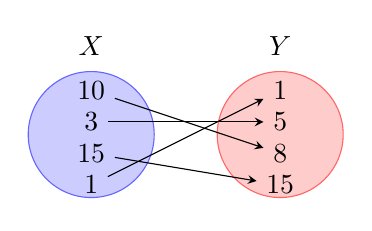
\begin{tikzpicture}[scale=0.8]
            \filldraw[fill=blue!20, draw=blue!60] (-1.5,0) circle (1cm);
            \filldraw[fill=red!20, draw=red!60] (1.5,0) circle (1cm);
        
            \node at (-1.5,1.4) {$X$};
            \node at (1.5,1.4) {$Y$};
        
            \node (x1) at (-1.5,0.7) {$10$};
            \node (x2) at (-1.5,0.2) {$3$};
            \node (x3) at (-1.5,-0.3) {$15$};
            \node (x4) at (-1.5,-0.8) {$1$};
            
            \node (y1) at (1.5,0.7) {$1$};
            \node (y2) at (1.5,0.2) {$5$};
            \node (y3) at (1.5,-0.3) {$8$};
            \node (y4) at (1.5,-0.8) {$15$};
        
            \draw[-stealth] (x1) -- (y3);
            \draw[-stealth] (x2) -- (y2);
            \draw[-stealth] (x3) -- (y4);
            \draw[-stealth] (x4) -- (y1);
        \end{tikzpicture}
        \caption{bijektiv}
        \label{subfig:bijektivDiagramm}
    \end{subfigure}
    \caption{Diagramm-Darstellung der Eigenschaften in \cref{definition:eigenschaftenFunktionen}}
    \label{fig:diagsurinjbi}
\end{figure} 

\noindent
Betrachten Sie \cref{fig:surinjbi}. Diese stellt die in \cref{definition:eigenschaftenFunktionen} beschriebenen Eigenschaften für eine Funktion $f:X\to Y$ schematisch dar. \cref{subfig:surjektiv} zeigt eine Funktion, die surjektiv, aber nicht injektiv ist, \cref{subfig:injektiv} eine Funktion, die injektiv, aber nicht surjektiv ist. Schliesslich wird in \cref{subfig:bijektiv} eine bijektive Funktion dargestellt. \cref{fig:diagsurinjbi} illustriert Surjektivität, Injektivität und Bijektivität für einfache Funktionen auf konkreten endlichen Mengen. Surjektivität, Injektivität und Bijektivität sind Eigenschaften, welche eine gegebene Funktion entweder haben kann oder nicht.

\subsubsection{Folgen}
\begin{definition}[Folge]{definition:Folge}
    Ist $X$ eine beliebige Menge und $f:\N\to X$ eine Funktion, welche auf $\N$ definiert ist und Werte in $X$ annimmt, dann wird $f$ eine \tib{Folge}\index{Folge} (in $X$) genannt. Ist $g:D\to X$ eine Funktion und $D\subsetneq\N$ eine endliche Teilmenge der natürlichen Zahlen, so wird $g$ \tib{endliche Folge}\index{Folge!endliche} in $X$ genannt.
\end{definition}
Häufig schreibt man $(x_n)_{n\in\N}, (x_n)$ oder auch $(x_0,x_1,x_2,\dots)$ für die Folge $f$. Dabei bezeichnet $x_n := f(n)$ das $n$-te \tib{Glied}\index{Folge!Glied einer} der Folge $f = (x_0,x_1,x_2,\dots)$ für jedes $n\in\N$. 
\beispiel{-}
{Die Funktion $f:\N\to\Z$ mit $n\mapsto 2n$ ist die Folge der geraden natürlichen Zahlen.} 

\section{Programmieren in Python}
Wir werden hier keine Einführung in die Python-Programmiersprache geben. Wir führen im Folgenden einige Details der Python-Sprache auf, welche wir in den Übungsaufgaben der nächsten Kapitel verwenden werden.
\begin{itemize}
    \item Der \tib{Modulo-Operator}\index{Modulo-Operator} \verb|%| (Prozent-Symbol) kann in der Form \verb|a % b| verwendet werden und liefert den ganzzahligen Rest bei der Division von \verb|a| mit \verb|b|. Beispielsweise sind die folgenden Ausdrücke wahr:
    \begin{center}
        \verb|7 % 3 == 1|, \quad \verb|5 % 8 == 5|, \quad \verb|22 % 4 == 2|, \quad \verb|42 % 6 == 0|.
    \end{center}
    Wir werden den Modulo-Operator zur Überprüfung auf Teilbarkeit verwenden. Denn \verb|b| ist offensichtlich genau dann ein Teiler von \verb|a|, falls \verb|a % b == 0| gilt.
    \item Eine Liste in Python wird durch eckige Klammern gekennzeichnet. Beispielsweise ist \verb|[3,2,2,7]| eine Liste mit $4$ Einträgen. Eine leere Liste (Liste ohne Einträge) wird durch \enquote{leere eckige Klammern} \verb|[]| bezeichnet. Mit dem Aufruf \verb|L.append(x)| wird ein Eintrag \verb|x| hinten (von rechts) in eine bereits bestehende Liste \verb|L| eingefügt (angehängt). Mit \verb|L[-1]| wird der letzte (am weitesten rechts stehende) Eintrag der Liste \verb|L| bezeichnet. Der Ausdruck \verb|L[:-1]| bezeichnet alle Einträge der Liste mit Ausnahme des letzten.
    \item In Python existiert die Möglichkeit, Argumenten einer Funktion ein \textit{Default-Argument} zu geben.
    \begin{lstlisting}[language=Python,caption=Default-Argument,numbers=none]
    # Default-Argument in Python
    def eineFunktion(a, b = 5):
        print(a + b)

    eineFunktion(3,6) # gibt den Wert 9 aus
    eineFunktion(3) # Aufruf mit Default-Argument b = 5: gibt den Wert 8 aus
    \end{lstlisting}
    Dieses Default-Argument wird genau dann verwendet, falls kein Wert für dieses Argument (explizit) angegeben wird.
    \item Die Operation \verb|math.ceil(x)| wird \textit{Aufrundungs-Operation} genannt und gibt die kleinste ganze Zahl, die grösser oder gleich \verb|x| ist. Beispielsweise gelten \verb|math.ceil(3.2) = 4| und \verb|math.ceil(3) = 3|. Um diese Operation verwenden zu können, muss die Bibliothek \verb|math| durch den Befehl \verb|import math| vor dem Gebrauch dieser Operation ins Programm eingefügt werden.
\end{itemize}
In \cref{listing:Vorwissen} haben wir die obigen Punkte noch einmal zusammengefasst.
\begin{lstlisting}[language=Python,caption=Vorwissen Python,label=listing:Vorwissen]
# gibt die durch 19 teilbaren Zahlen in {0,1,2,...,99} aus:
for k in range(100):
    if (k % 19) == 0:
        print(k) # gibt aus: 0 19 38 57 76 95

# Listen
L = [3, 7, 2, 3]
L.append(99) # L ist nun [3, 7, 2, 3, 99].
print(L[-1]) # gibt aus: 99
print(L[:-2])# gibt aus: 3, 7, 2

# Default-Argument
def person(vorname, nachname = 'Nachname unbekannt', alter = '-'):
    print('Vorname: ', vorname, ', ' , 'Nachname: ', nachname, ', ', 'Alter: ', alter, sep='')

person('Sandra') # gibt aus: Vorname: Sandra, Nachname: Nachname unbekannt, Alter: -

person('Toni', 'Wildeisen') # gibt aus: Vorname: Toni, Nachname: Wildeisen, Alter: -

# Importieren einer Bibliothek und Verwendung der Aufrundungs-Funktion
import math # Einfügen der Bibliothek 'math'
print(math.ceil(3.00002)) # gibt aus: 4
\end{lstlisting}